\chapter{O CERN e Física Experimental de Altas Energias}

Neste capítulo estão descritos com maiores detalhes o contexto no qual o
trabalho está inserido. Serão introduzidos o estudo de Física de Partículas
Elementares e o Modelo Padrão (seção \ref{sec:fis_part}),
 o experimento LHC (seção~\ref{sec:lhc}), o detetor ATLAS 
(seção~\ref{sec:ATLAS}), e o ferramental utilizado pela colaboração
(seção~\ref{sec:ferramentas}). 

\section{Introdução a Física das Partículas Elementares}
\label{sec:fis_part}

A ciência é uma ferramenta que busca entender fenômenos e ser capaz de
prêver o seu comportamento. A física busca atualmente criar um único 
modelo capaz de explicar as interações que ocorrem no universo. O modelo mais
próximo de realizar tal tarefa está imbutido no estudo da Física das
Partículas Elementares. 

Se dá o nome de Física de Partículas Elementares ao estudo dos contituintes
elementares e da natureza do universo. Embora a noção de que a matéria é
composta por um conjunto de constituintes elementares tenha surgido em cerca de
430 a.C., por Demócritos \cite{democritos}, o seu estudo na ciência moderna teve ínicio no século
19, quando o elétron foi descoberto por Thompson \cite{eletron}.
Uma das grandes conquistas do século 20 foi o desenvolvimento do Modelo Padrão
de Física de Partículas Elementares. 
Esse modelo descreve de maneira bem
sucedida as relações entre
partículas elementares conhecidas pela ciência atual \cite{introduction_particle_physics} e as características de
três das quatro forças conhecidas que interagem com essas partículas:
eletrogmagnetismo, forças fracas e forças fortes. Apesar de esforços, não se 
foi capaz de incluir no modelo, até o momento, a força gravitacional \cite{natureza_do_universo}.

O Modelo Padrão utiliza 12 partículas elementares divididas em dois grupos, os
léptons e os quarks, e 4 partículas transportadoras de força. São parâmetros a
serem determinados experimentalmente a energia, o
A Figura \ref{fig:modelo_padrao} contêm as diferentes partículas que são
descritas pelo Modelo Padrão.

\begin{figure}[h!t]
\centering
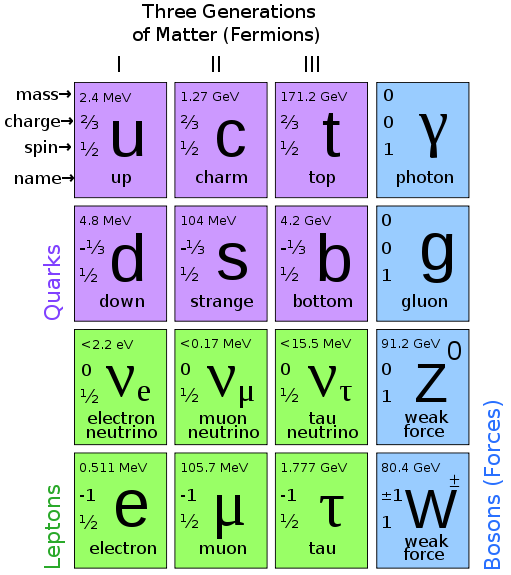
\includegraphics[width=0.6\textwidth]{imagens/standart_model.pdf}
\caption{O Modelo Padrão de partículas elementares. Extraído de
\cite{wiki_standart_model}.}
\label{fig:modelo_padrao}
\end{figure}

Existem três diferentes gerações de partículas elementares, cada uma com maior
massa e carga. Para cada geração existem um par de quarks, onde um dos
constituintes do par tem carga positiva e o outro negativa: \emph{up} e
\emph{down}, \emph{charm} e \emph{strange}, \emph{top} e \emph{bottom}.

O grupo dos léptons pode ser subdividido em dois grupos, um com carga e massa, contendo
o elétron, múon e táon, e outro sem carga e massa reduzida contendo o
neutrino do elétron, neutrino do múon e neutrino do táon.

Além dessas partículas elementares, também foi verificada a existência das suas
anti-partículas, ou seja, partículas com as mesmas massas, mas
carga e momento angular invertidos. Normalmente elas são 
representadas através de uma barra por cima dos simbúlas das partículas, exceto
para os léptons elêtron, múon e táon, onde apenas os sinais da carga são
modificados. A anti-partícula do elétron tem o nome de pósitron, por motivos
históricos.

As forças são comunicadas através das partículas elementares através da troca de
partículas transportadora de força, chamadas de bóssoms, que carregam uma
quantidade discreta de energia de uma partícula a outra. Cada força tem seus
bóssoms característicos: o glúon (força forte), o fóton (força magnética) e os
bóssoms W e Z (força fraca). Os físicos esperam adicionar a força gravitacional
através da partícula \emph{graviton}.

Os quarks sofrem influência de todas as forças descritas pelo Modelo Padrão.
Nenhum dos léptons sofrem interações com os glúons, portadores da força forte, e
os léptons neutrinos tambêm não interagem com a força eletromagnética (fótons), uma vez
que não tem carga, sendo por esse motivo muito dificeis de serem identificados
já que só interagem com a força fraca.

Para distâncias maiores que $10^{-13}$ cm a força eletromagnética é dominante,
enquanto para distâncias menores, as interações forte e fraca se destacam. A
intensidade relativa (em comparação com a interação forte) dos quatro tipos de
interação é mostrada na Tabela \ref{tab:interacoes}.

\begin{table}
\centering
\begin{tabular}{cc}
\hline
\textbf{Interação} & \textbf{Intensidade Relativa} \\
\hline
Forte & 1 \\
Eletromagnética & $10^{-2}$ \\
Fraca & $10^{-5}$ \\
Gravitacional & $10^{-39}$ \\
\hline
\label{tab:interacoes}
\end{tabular}
\caption{Intensidade Relativa (em comparação com a interação forte) dos diversos
tipos de interação. Extraído de \cite{tese_eduardo}.}
\end{table}

Uma formulação atualmente aceita pela física teórica (conhecida como \emph{Gauge
Invariance} prevê que todas as partículas tem massa de repouso nula. Foi
introduzido um mecânismo, por Peter Higgs em 1964, para corrigir o Modelo Padrão de modo que ele atendesse
a essa formulação, conhecido como o bóssom de Higgs. O bóssom de Higgs seria
uma partícula mediadora responsável de fornecer massa às partículas elementares.
A existência do bóssom de Higgs é a mais importânte previsão do Modelo Padrão
ainda não verificada experimentalmente e sua busca é de máxima importância para
a física de partículas \cite{tese_eduardo}.

De acordo com a Teoria da Relatividade, não há diferença qualitativa entre
massa e energia, está diferença é apenas quantitativa \cite{einstein} sendo descrita por:
\begin{equation}
E=m_0c^2
\end{equation}
onde E é a energia, $m_0$ a massa de repouso e c uma constante que representa a
velocidade da luz no vácuo, aproximadamente $3\times 10^{8}$. Desta forma, a
única diferença quando refere-se a massa é que está se referindo a uma grande
quantidade de energia. Assim, ao se acelerar partículas de menores energias é
possível, através da interação causada pela colisão, criar novas partículas de
maiores energias.

Na próxima seção será apresentado o acelerador de partículas LHC, que 
atinge energias nunca antes alcançadas experimentalmente,
esperando criar condições para a geração do bósson de Higgs.

\section{O Large Hadron Collider}
\label{sec:lhc}

O CERN ({\it Centre Européene pour la Rechèrche Nucleaire}) é o maior
laboratório de física de partículas do mundo, situado na fronteira da Suíça com
a França, contando com a colaboração de cientistas vindos de institutos
do mundo todo. Desde sua fundação em 1954, tem sido uma das referências de
avanços tecnológicos. Dentre seus feitos constam a construção do primeiro 
colisionador de prótons-prótons (1971), a descoberta 
da corrente de neutrons (1973) e das partículas Z e W (1983), 
e a invenção da Web (1990) \cite{webCERN}.

Atualmente, o CERN está engajado no projeto LHC (Large Hadron
Collider), um acelerador de partículas circular de 27 quilômetros de
circunferência, situado entre 50 a 175 m debaixo do solo. 
No atual momento, ele realiza colisões de pacotes de prótons a uma energia
de 7 TeV no centro de massa, que serão expandidos a 14 TeV em 2013 \cite{webATLASa}.
O LHC apresenta uma oportunidade sem precedentes para provar o domínio da
nova física na região TeV e lançar luz sobre algumas das questões fundamentais
não resolvidas da física das partículas elementares \cite{hunt_for_physics}. 

Para desenvolver a altíssima energia necessária para o experimento o CERN 
utiliza outros aceleradores construídos anteriormente, acelerando os feixes de prótons até atenderem
a energia desejada para a colisão. Na Figura \ref{fig:esquema_aceleradores} pode-se observar
o esquema de aceleração de prótons, inicia-se na extração de prótons de átomos
de hidrogeneo que são levados ao LINAC 2, um acelerador linear,
que inicia a sequencia de aceleração. Em seguida são utilizados os aceleradores
circulares BOOSTER, PS, SPS, até finalmente abastecer o LHC com os feixes de
prótons.

\begin{figure}[h!t]
\centering
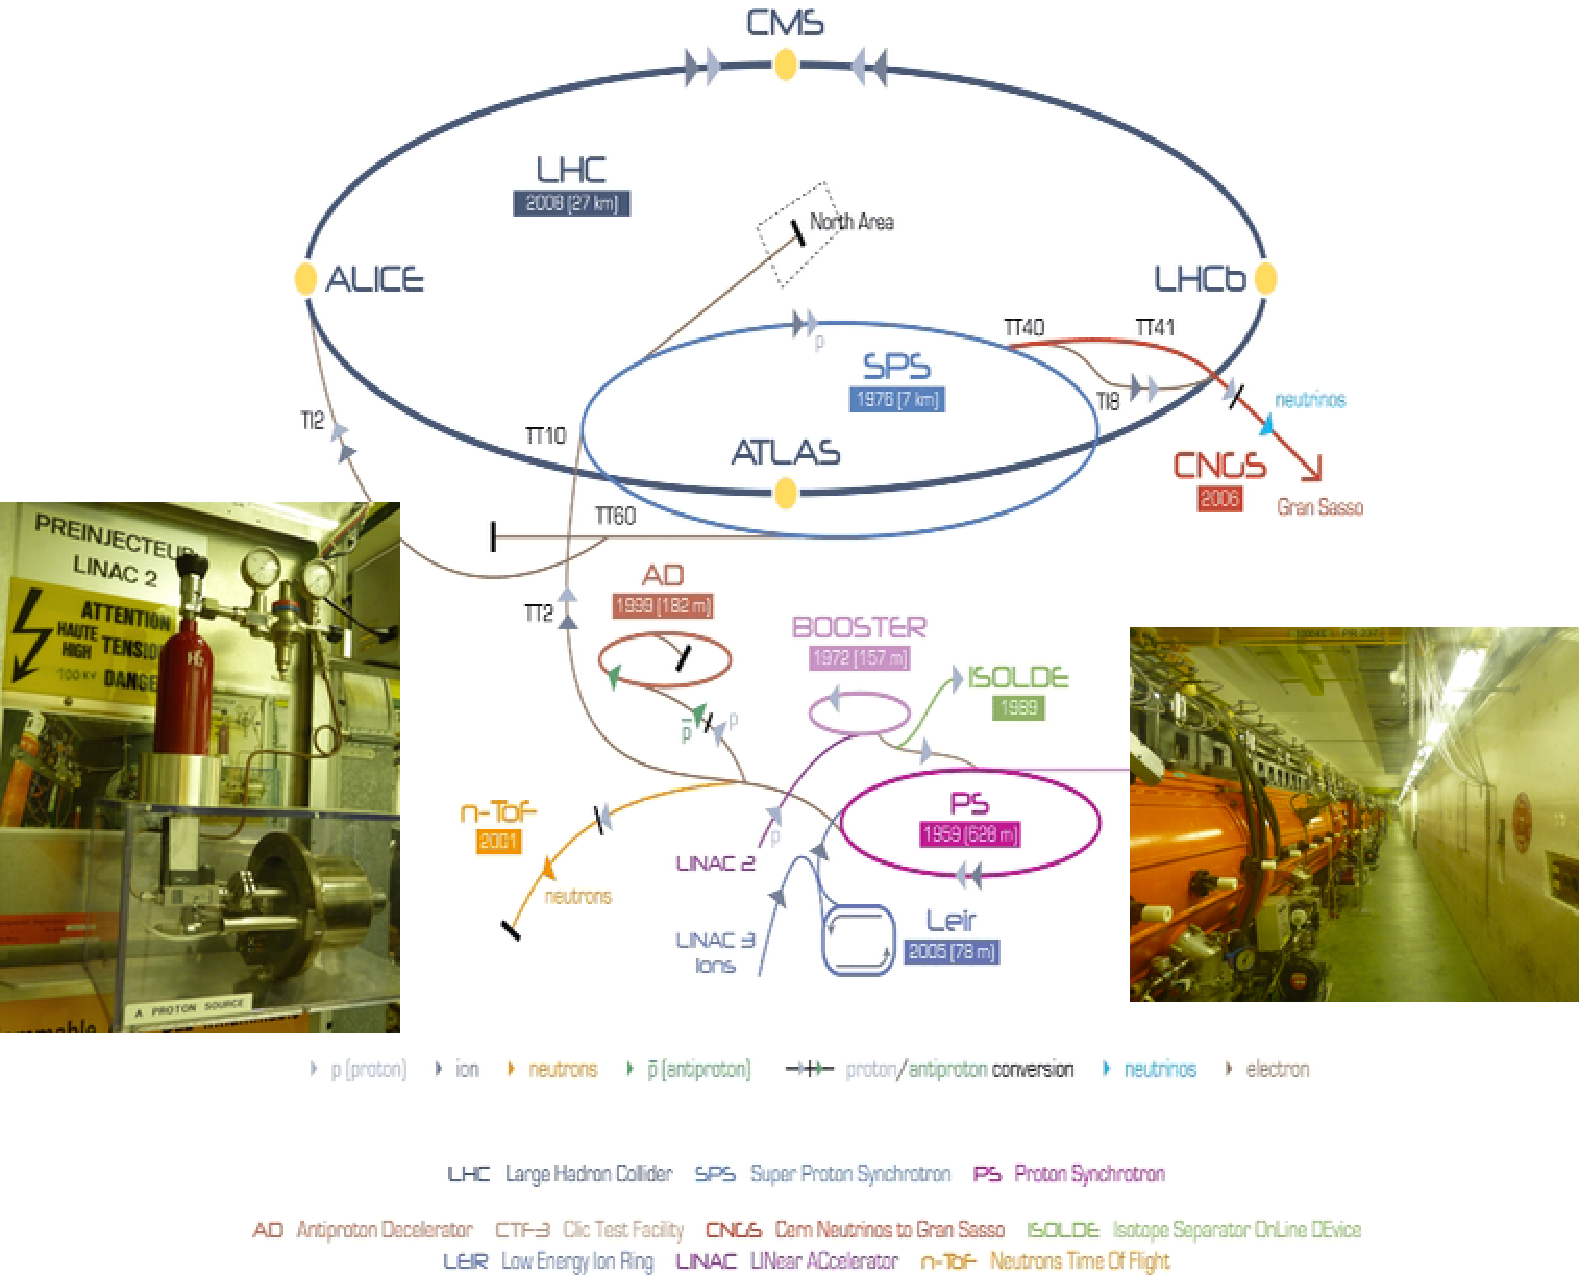
\includegraphics[width=\textwidth]{imagens/lhc_garrafa_linac2.pdf}
\caption{Os diferentes aceleradores e detectores do CERN, extraido de
\cite{cern_accelerators}. A seta cinza claro corresponde ao sentido do
deslocamento de prótons nos aceleradores. À esquerda, foto da garrafa
de onde são retirados os prótons, e na direita foto do LINAC 2.}
\label{fig:esquema_aceleradores}
\end{figure}

Tão importante quanto obter altas energias, é obter alta
luminosidade, um indicador da concentração 
de partículas no feixe. A luminosidade é definida como:
\begin{equation}
L=fn\frac{N_1 N_2}{A}
\label{eq:luminosidade}
\end{equation}
onde a frequência de cruzamento entre feixes\footnote{Do
inglês \emph{bunch crossing rate}}, f, é de 
40 MHz, n é o número de feixes, $N_i$ equivale ao número de prótons em
cada pacote, correspondentes a $1.5\times10^{11}$ no início de uma
temporada\footnote{Em inglês utilizam o termo \emph{run}} de colisão nominal, e,
finalmente, o termo A é a área dada pela secção transversal do feixe, do tamanho
de um fio de cabelo (64 microns) no ponto de interação \cite{webLHC}. No LHC se
irá atingir uma luminosidade até $10^{34}cm^{-2}s^{-1}$.

O número de colisões é diretamente proporcional a luminosidade, o que explica
desejar-se elevadas luminosidades. A taxa de colisão é definida por
\cite{ATLAS_TDR}:
\begin{equation}
R = L \times \sigma
\label{eq:taxa_colisao}
\end{equation}
onde L é a luminosidade e $\sigma$ é a seção eficaz \cite{wiki_cross_section},
expressa em mbarns. Para as colisões a 7 TeV a seção eficaz é de 110 mbarn, e
60mbarn para o caso de colisões inelásticas.
Nesses valores se obtêm 19 eventos de colisão inelásticas para cada
cruzamento de feixes \cite{webLHC}.

Os eventos de colisões podem ser de dois tipos \cite{THESIS_LAR}:

\begin{enumerate}
\item \textbf{Colisões Rigidas}:
elas são devidas as interações de curto alcance,
resultando em grandes transferências de momemnto que produzindo partículas de
alto momento, assim como condições para a geração de novas partículas de altas
energias, como o bóssom de Higgs.
\item \textbf{Colisões Suaves}: 
é o tipo de iteração mais comum e devidas as interações de longo alcance entre dois prótons cruzantes. Os
resultados são partículas com grande momento longitudinal\footnote{Na direção de
propagação do feixe} e pouco momento transverso\footnote{Perpendicular à
propagação}. Esses eventos de colisão são
denominados de \emph{mininum bias} e são compostos na sua maioria por jatos.
\end{enumerate}

O experimento LHC conta com quatro detectores de maior escala: ATLAS, CMS, ALICE e
LHCb; e dois de menor escala: TOTEM e LHCf. O trabalho atual está definido no
escopo da colaboração do detector ATLAS, onde o mesmo é definido com maiores
detalhes na seção~\ref{sec:ATLAS}.

O ATLAS e o CMS são de propósito geral, ou seja, são capazes de estudar diversos
fenômenos físicos. O fato de existirem dois detectores projetados de forma
diferente, mas para o mesmo fim, é importante para que um possa confirmar o
resultado do outro.

O LHCb é um detector especializado no estudo do quark \textit{beauty} com o
intuito de investigar a diferença entre matéria e antimatéria.

O ALICE, por sua vez, estudará o plasma quark-gluon que será formado quando o
LHC fizer colisões de íons de chumbo, recriando as condições que existiram
instantes após o Big Bang.

Os dois menores detectores são o LHCf e o TOTEM. O LHCf, que se situa na mesma
caverna do ATLAS, estuda o comportamento de raios cósmicos, utilizando
partículas que não chegaram a colir no ponto de colisão, mas foram desviadas.
O TOTEM, que está instalado perto do CMS, estuda o feixe de prótons produzidos
pelo LHC, bem como a estrutura interna do próton.

\section{O Detector de Partículas ATLAS}
\label{sec:ATLAS}

O ATLAS (\textit{A Toroidal LHC Apparatus}) é o maior dos detectores que operam
no LHC, medindo 45 metros de comprimento e 25 metros de altura e largura. Como é
um detector de propósito geral, o detector registra dados sobre os eventos de
colisões de partículas que podem ser usados para estudos em diversas áreas da
física. 

O experimento está na fase de operação desde setembro de 2008 \cite{webLHCFirstBeam},
quando o primeiro feixe de partículas circulou no acelerador e os primeiros
eventos de colisão dos prótons com moléculas de gás dentro do tubo do acelerador
foram registrados. Para coletar dados suficientes para as análises físicas o
experimento pode durar cerca de 20 anos \cite{ATLAS_TDR}.

O ATLAS foi construído e é operado por uma colaboração internacional envolvendo
cerca de 2500 físicos de mais de 169 instituições e laboratórios de 37 países
\cite{webATLAS}. Esses números incluem a UFRJ, que participa através da COPPE,
da Escola Politécnica e do Instituto de Física. O detector é composto por 4
sub-detectores: o Inner detector, detector de traço; o Liquid Argon, que é o
calorímetro eletromagnético; o Tile Calorimeter, que é o calorímetro hadrônico,
e o Muon Spectrometer responsável por realizar medições sobre os múons. Cada uma
dessas partes teve seus componentes construídos por um grupo diferente,
pertencente às instituições colaboradoras.  Uma vez construídos e testados, os
componentes foram levados ao CERN, onde foram instalados em seus lugares
definitivos. Para coordenar essa montagem e fornecer a infra-estrutura
necessária no local do experimento, existe o grupo da Coordenação Técnica
({\it ATLAS Technical Coordination}).

\section{Ferramentas Utilizadas na Colaboração}
\label{sec:ferramentas}

